\chapter{Performance}
\label{chap:performance}
\section{Computational Efficiency}
\label{sec:performance_computationalefficiency}

\subsection{Evaluation}
\label{sec:performance_computationalefficiency_evaluation}

In Utility Designer, the best state is decided at each evaluation tick. The tick rate can be set in the UtilityDesigner script and is clamped between 0.01s and 1s. Alternatively, Unity's update method can be used. This allows for a custom balance between the NPC's reaction time, in terms of switching to the right state faster, and performance. The question now is how expensive such an evaluation tick is:

On every evaluation tick, the code loops over all states. It immediately jumps to the next state if the state is not "Active". It loops over all preconditions and returns as soon as one of them is not met. Only when all preconditions are met does it loop over the evaluators to calculate their scores.

Scoring an evaluator means obtaining the current value of its curve based on its consideration. This score is then added to the base score, multiplied by its weights and clamped between the minimum and maximum scores if the appropriate switches are set. When it comes to calculating the weights for each evaluator, the calculation of the percentages only needs to be done once, at the start of the programme.

All states are ranked according to their score. After getting the best state, there is a chance that this state will not be chosen, based on the "Fail Chance". If the state fails, the next best state is chosen and the fail chance is also checked. This happens for all states until the state does not fail or it is the last state left. Since the states are already ordered, choosing the next best state just means looking at the next element in the list, and is therefore very efficient.

The considerations are also updated at the same tick rate, changing their value according to "Change Per Sec". They are always updated just before the evaluation takes place, to ensure that their value is up to date when the evaluation takes place.

\subsection{Execution}
\label{sec:performance_computationalefficiency_execution}

Similarly to the evaluation, the behaviour tree is updated on every execution tick, according to the settings in the UtilityDesigner script. It is also clamped between 0.01s and 1s, with the option to use Unity's Update method instead. A faster tick rate makes the NPC's behaviour more responsive, while a lower tick rate offers better performance.

\newpage

On each execution tick, the root node of the currently executing state is updated, all other behaviour trees of other states are ignored. Updating the behaviour tree does NOT mean looping over all nodes, it only updates the currently executing path. The composite node, which is the only node type that can have multiple children, caches the last child that returned Running. Each time the node is updated, it will only update the relevant child, without looking at the others. This is of course slightly different for the Parallel node, which can have multiple running children, and therefore needs to update them all on every tick.

\section{Profiling}
\label{sec:performance_profiling_profiling}

Unity provides a tool called the Profiler, which helps to analyse the efficiency of the game. To further test the performance of Utility Designer, the daily routine scene was populated with 1000 agents, each with their own local consideration set, but all sharing the same UtilityBehaviour. This means that they all make decisions on their own, but only share the same behaviour logic. The tick rate of the evaluation is set to 0.1s and for the execution tab it is set to Unity's Update method for each agent. An Intel Core i7 12700KF CPU was used for these tests.

\begin{figure}[H]
	\centering
		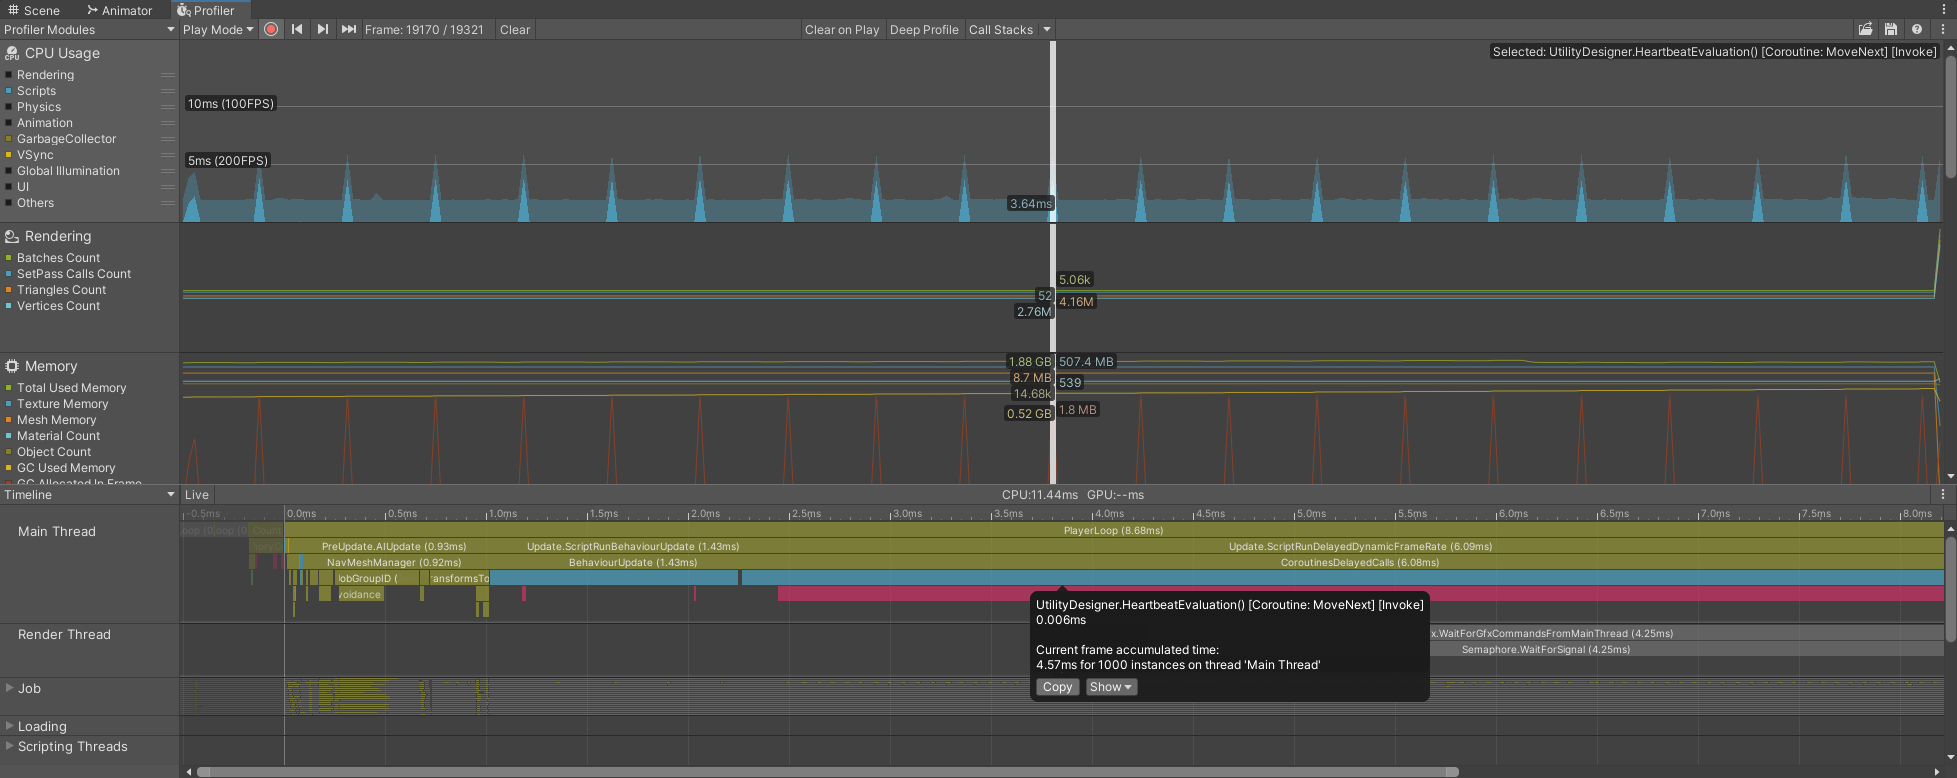
\includegraphics[scale=0.302]{images/utility_designer_profiling_1.png}
	\caption{Profiler with evaluation tick rate = 0.1s and execution tick rate = update}
	\label{fig:utility_designer_profiling_1}
\end{figure}

The first curve in light blue shows the CPU usage of the scripts. The tick rate of the evaluation tab is easy to see with spikes every 0.1s. Hovering over one of these spikes shows the exact time it takes to evaluate all 1000 agents in the main thread, which is 4.57ms. This time will change as states or evaluators are added or removed. Reducing the tick rates of Utility Designer will result in better performance:

\begin{figure}[H]
	\centering
		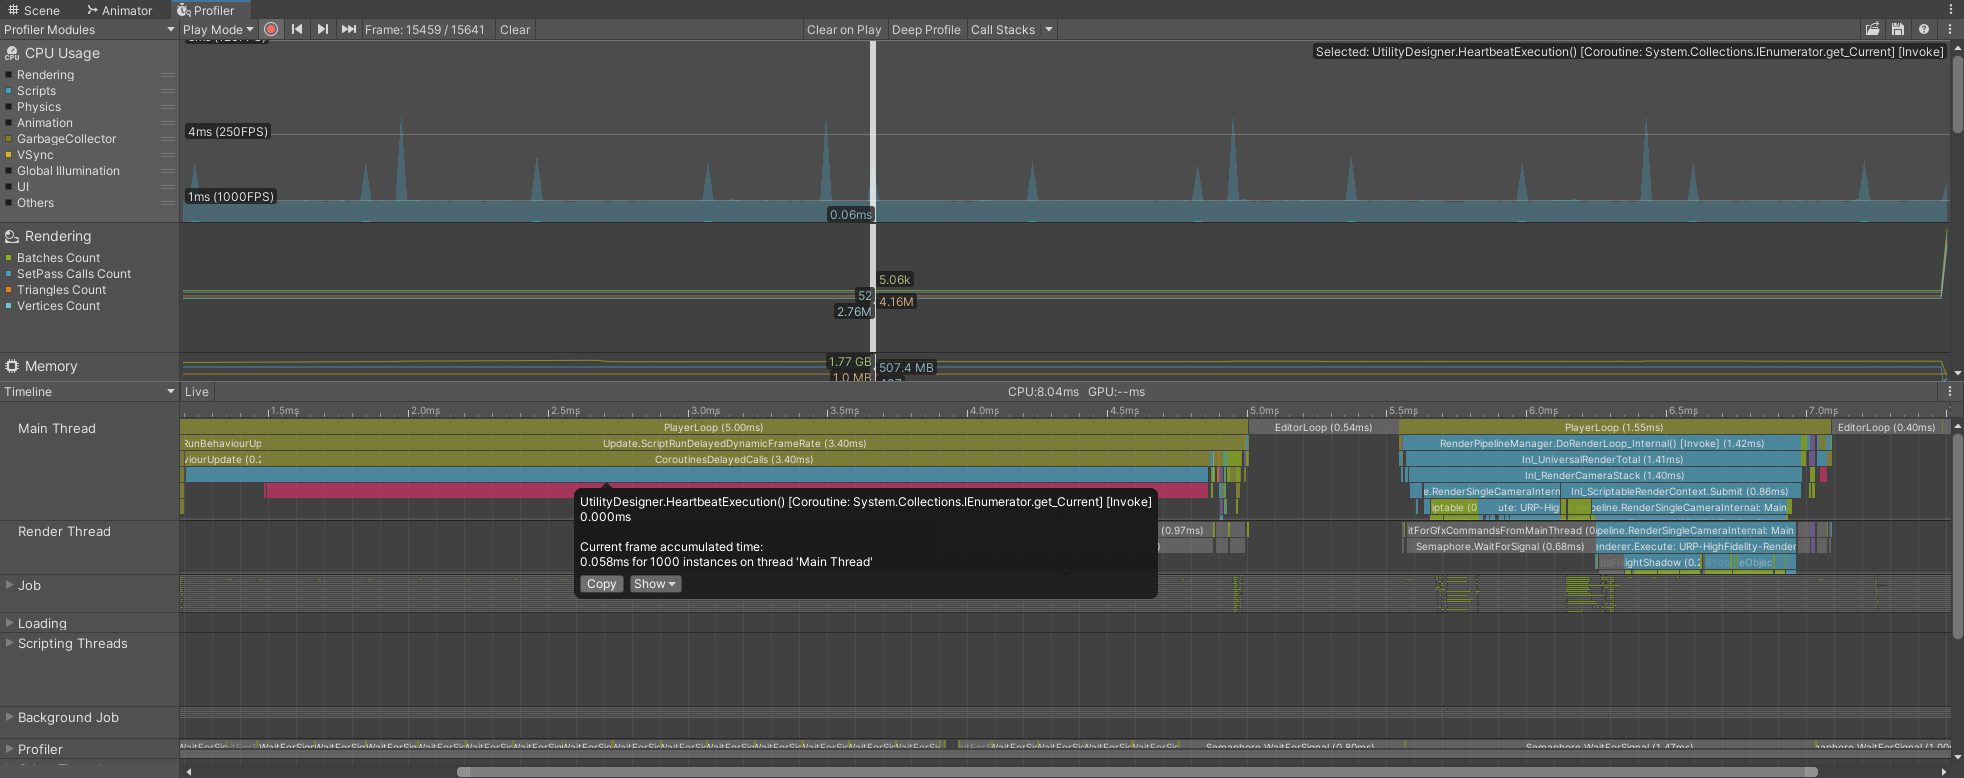
\includegraphics[scale=0.302]{images/utility_designer_profiling_2.png}
	\caption{Profiler with evaluation tick rate = 0.5s and execution tick rate = 0.2s}
	\label{fig:utility_designer_profiling_2}
\end{figure}

Looking at this example, it is clear that some performance can be gained by reducing the tick rates. The evaluation tick rate is set to 0.5s and is represented by the larger spike in figure \ref{fig:utility_designer_profiling_2}, while the execution tab is set to 0.2s and represents the smaller spikes. In the example of the daily routine scene, an execution tick is less expensive than an evaluation tick with a total of 0.058ms for 1000 agents. Overall, it still seems to be able to maintain a fairly high frame rate with 1000 fps down to around 200 fps at the exact time of the evaluation tick in the Unity editor. Often a built game will have an even higher frame rate than when running in the Unity editor.